\documentclass[declaration,shortabstract]{iithesis}

\usepackage[utf8]{inputenc}

\polishtitle    {Implementacja wydajnych struktur danych\fmlinebreak do~praktycznych operacji na~słowach}
\englishtitle   {Implementation of efficient data structures\fmlinebreak for practical string operations}
\polishabstract {Przedstawiona praca opisuje zaimplementowane programy, które realizują praktyczne operacje na tekście. W programach zostały zaimplementowane zarówno klasyczne algorytmy, jak i pomysły na rozwiązanie podanego problemu, które pojawiły się w przeciągu kilku ostatnich lat jako naukowe publikacje. Część z tych pomysłów została odpowiednio uproszczona, aby implementacja w rozsądnym czasie była możliwa. Poprawność i czas działania wszystkich zmian względem oryginalnych wersji została udowodniona. Pracę uzupełnia analiza wydajności i poprawności przedstawionych programów.}
\englishabstract{This paper describes the implemented programs, which realize practical text operations. In these programs, there were implemented both classic algorithms and new ideas, which appeared in the past few years as published papers. Some of them were properly simplified, so they could be implemented in a reasonable time. Correctness and complexity of all changed things was proven. In the last part of this paper, I~have analyzed the performance and correctness of the given programs.}
\author         {Michał Górniak}
\advisor        {dr Paweł Gawrychowski}
\date          {11 września 2020}                     
\transcriptnum {299883}
\advisorgen    {dr. Pawła Gawrychowskiego}

\usepackage{tikz,graphicx,listings,amsthm,mathtools,array,caption,forest,comment,bbold}

\theoremstyle{definition} \newtheorem{definition}{Definicja}[chapter]
\theoremstyle{remark} \newtheorem{remark}[definition]{Obserwacja}
\theoremstyle{plain} \newtheorem{theorem}[definition]{Twierdzenie}
\theoremstyle{remark} \newtheorem{example}{Przykład}[definition]
\theoremstyle{plain} \newtheorem{lemma}[definition]{Lemat}

\usetikzlibrary{shapes.geometric}
\forestset{%
  default preamble={
    for tree={
      circle,
      draw,
      inner sep=0pt,
      minimum size=1cm,
      font=\scriptsize,
      edge=->,
      anchor=north
    }
  },
  ssarbre/.style={isosceles triangle,
                  draw,
                  shape border rotate=90,
                  minimum size=2cm,
                  child anchor=apex,
                  anchor=apex}
}

\begin{document}

\chapter{Wprowadzenie}

Algorytmy tekstowe są~niewątpliwie dziedziną algorytmów, która ma wiele praktycznych zastosowań. Wiele programów komputerowych, takich jak edytory programistyczne czy edytory tekstu, operują na~tekście oraz bazują na~jego ciągłej modyfikacji. Łączy się to~najczęściej z~potrzebą wykonywania pewnych typów zapytań dotyczących aktualnego stanu tekstu, takich jak wyszukiwanie wystąpień wybranego fragmentu czy porównywanie leksykograficzne dwóch fragmentów tekstu. Z drugiej strony, z~algorytmicznego punktu widzenia, na~każdy ciąg znaków, nie tylko alfanumerycznych, możemy popatrzeć jak na~tekst. W związku z~tym możemy jako tekst interpretować chociażby pliki komputerowe zapisane binarnie, stąd też popularnym tematem rozważań naukowców są algorytmy kompresji tekstu.

Przy analizie opisywanych algorytmów, w~pierwszej kolejności będziemy zwracać uwagę na~ich czas działania, a~w~drugiej kolejności na~zużycie pamięci. Niektóre z~analizowanych w~pracy algorytmów będą korzystały z~liczb losowych. W przypadku takich algorytmów będziemy musieli zdefiniować, jak tak naprawdę szacujemy czas działania takiego programu. Zostanie to~dokładniej opisane w~jednym w~kolejnych rozdziałów pracy.

Opiszmy zatem dosyć wysokopoziomowo analizowany w~tej pracy problem. Wyobraźmy sobie, że utrzymujemy w~pewnej strukturze danych zbiór słów, gdzie słowem jest po~prostu ciąg znaków, niekoniecznie alfanumerycznych. Chcemy móc modyfikować ten zbiór, to~znaczy móc realizować następujące operacje: 
\begin{itemize}
    \item dodać do~niego nowe słowo, 
    \item złączyć dwa już istniejące w~zbiorze słowa,
    \item wybrać słowo ze zbioru, pociąć je na~dwa słowa względem pewnej pozycji, a~następnie oba słowa dodać do~naszego zbioru. 
\end{itemize}
Za każdym razem gdy prosimy naszą strukturę danych o~wykonanie którejś z~wyżej wspomnianych operacji, struktura ta wyda nam etykiety nowo dodanych słów. Możemy sobie wyobrażać, że te etykiety są bardzo małe, bo słowa które mogą powstać w~wyniku tworzenia tych operacji, mogą szybko stać się bardzo długie. W każdym momencie możemy również zapytać o~coś naszą strukturę. Każde pytanie wygląda tak, że przekazujemy strukturze danych dwie etykiety, a~ona może nam odpowiedzieć na~jedno z~zapytań, dotyczące słów które kryją się za tymi etykietami:
\begin{itemize}
    \item czy słowa te są równe,
    \item czy pierwsze ze słów jest mniejsze leksykograficznie od drugiego,
    \item jak dużo początkowych liter w~jednym i~drugim słowie jest takich samych.
\end{itemize}

Z początku może się wydawać, że opisane wyżej operacje nie są zbyt praktyczne. Zobaczmy jednak jak możemy przy ich pomocy realizować niektóre zaawansowane zadania edytora tekstu. Powiedzmy, że chcemy umieć zaznaczać fragment tekstu i~go skopiować w~inne miejsce lub wyciąć i~wkleić w~inne miejsce, lub całkowicie usunąć. Możemy też zaznaczać dwa wybrane elementy i~pytać czy są takie same lub gdzie jest pierwsza pozycja niezgodności między tymi fragmentami. Opiszę jak przy pomocy operacji naszej struktury danych, można wykonać te zapytania.

Utrzymujemy etykietę tekstu z~edytora. Gdy chcemy operować na~wybranym fragmencie, to~możemy najpierw wykonać dwa cięcia, jedno przed początkiem, a~drugie zaraz za zakończeniem i~w ten sposób otrzymamy trzy etykiety, oznaczające podział tekstu na:
\begin{enumerate}
    \item część przed wybranym fragmentem,
    \item wybrany fragment,
    \item część za wybranym fragmentem.
\end{enumerate}
Teraz usunięcie fragmentu to~złączenie części (1) oraz (3) oraz przyjęcie za nową etykietę całego tekstu etykiety z~tego złączenia. Kopiowanie fragmentu to~cięcie etykiety tekstu w~miejscu, gdzie chcemy wkleić wybrany fragment, a~następnie zrobienie dwóch złączeń z~etykietą (2). Natomiast wycinanie i~wklejanie w~innym miejscu, to~połączenie dwóch poprzednio opisanych sposobów.

Aby realizować zapytania, postępujemy analogicznie. Poprzez cięcia wybieramy etykiety dwóch wybranych fragmentów, a~następnie używamy na~nich odpowiadającego zapytania z~naszego algorytmu. Pierwsza niezgodność to~tak naprawdę powiększony o~jeden wynik zapytania do~struktury o~to, jak dużo początkowych liter w~jednym i~drugim słowie jest takich samych.

Powyższy przykład pokazuje jedno z~praktycznych zastosowań interfejsu opisanej struktury danych. Okazuje się również, że wspomniane operacje są w~stanie realizować dużo bardziej skomplikowane zapytania dotyczące utrzymywanego zbioru słów. Staje się to~dobrą motywacją do~analizowania tego problemu. 

W kolejnych rozdziałach pracy opiszę dokładnie definicję naszego problemu oraz kilka implementacji struktur danych realizujących podany interfejs. Ważną częścią pracy będzie analiza złożoności czasowej i~pamięciowej operacji na~zaimplementowanych strukturach. Z drugiej strony postaram się położyć nacisk na~rozwiązania technicznych aspektów implementacji, zwłaszcza w~tych miejscach, gdzie użyty sposób implementacji odbiega od klasycznego lub żadna implementacja danego algorytmu w~ogóle nie istniała.

Na końcu pracy przeanalizuję prawdziwe czasy działania zaimplementowanych struktur, aby porównać je z~czasami asymptotycznymi i~sprawdzę dla różnych rozmiarów danych oraz zapotrzebowań na~wybrane operacje, która z~implementacji działa najszybciej, a~która zużywa najmniej pamięci. Opiszę również sposób testowania poprawności zaimplementowanych programów.

\chapter{Definicje i~formalny opis problemu}

\section{Definicje}

Na początek opiszę ogólne definicje używane w~algorytmach tekstowych.

\begin{definition}
    \textit{Alfabetem} (z reguły oznaczanym przez $\Sigma$) nazywamy skończony zbiór znaków.    
\end{definition}

\begin{definition}
    \textit{Słowem} nad alfabetem $\Sigma$ nazywamy skończony uporządkowany ciąg znaków z~tego alfabetu. Notacja $w = w_1 w_2 \ldots w_{n}$ oznacza słowo $w$ składające się z~$n$ znaków odpowiednio $w_1, w_2, \ldots, w_{n}$. Długość słowa $w$ oznaczamy przez $|w|$.
\end{definition}

\begin{example}
    Dla alfabetu $\Sigma = \{a, b\}$, słowami są między innymi $a$, $bba$, $baba$, $bbbbbbbb$.
\end{example}

\begin{definition}
    Dla alfabetu $\Sigma$ przez $\Sigma^*$ oznaczamy zbiór wszystkich słów nad alfabetem $\Sigma$, w~szczególności słowo puste, oznaczane symbolicznie jako $\epsilon$, a~przez $\Sigma^+$ oznaczamy $\Sigma^* \setminus \{ \epsilon \}$.
\end{definition}

\begin{definition}
    \textit{$(i, j)$-podsłowem} słowa $w = w_1 w_2 \ldots w_{n}$ dla $1 \leq i~\leq j \leq n$ nazwiemy słowo $w_i w_{i+1} \ldots w_{j-1} w_j$, zapisywane też czasem symbolicznie jako $w_{i \ldots j}$.
\end{definition}

\begin{definition}
    Słowo $u$ jest podsłowem słowa $w$, jeśli $u$ jest $(i, j)$-podsłowem słowa $w$ dla pewnych $i, j$.
\end{definition}

\begin{example}
    Podsłowami słowa $bananowy$ są między innymi $banan$, $nano$, $nowy$, ale $banowy$ nie jest podsłowem słowa $bananowy$.
\end{example}

\begin{definition}
    \textit{$i$-prefiksem} słowa $w$ nazwiemy $(1, i)$-podsłowo słowa $w$, zapisywane też czasem symbolicznie jako $w_{\ldots i}$. Przyjmujemy też, że $0$-prefiksem jest słowo puste.
\end{definition}

\begin{definition}
    Słowo $p$ jest \textit{prefiksem} słowa $w$, jeśli $p$ jest $i$-prefiksem słowa $w$ dla pewnego $i$.
\end{definition}

\begin{example}
    Wszystkimi prefiksami słowa $koc$ są $\epsilon$, $k$, $ko$, $koc$.
\end{example}

\begin{definition}
    \textit{i-sufiksem} słowa $w$ długości $n$ nazwiemy jego $(i, n)$-podsłowo, zapisywane też czasem symbolicznie jako $w_{i \ldots}$. Przyjmujemy też, że $(n+1)$-prefiksem jest słowo puste.
\end{definition}

\begin{definition}
    Słowo $s$ jest \textit{sufiksem} słowa $w$, jeśli $s$ jest $i$-sufiksem słowa $w$ dla pewnego $i$.
\end{definition}

\begin{example}
    Wszystkimi sufiksami słowa $koc$ są $\epsilon$, $c$, $oc$, $koc$.
\end{example}

\begin{definition}
    Dla uporządkowanej pary słów $(w, v)$, ich \textit{konkatenacją} nazwiemy słowo powstałe poprzez sklejenie tych dwóch słów ze sobą zgodnie z~kolejnością pary. Konkatenację taką zapisujemy symbolicznie jako $wv$.
\end{definition}

\begin{example}
    Konkatenacją słów $nie$ oraz $zdrowy$ jest słowo $niezdrowy$.
\end{example}

\section{Formalny opis problemu}

W tym podrozdziale sformalizuję opisany we wprowadzeniu problem. Mamy dany ustalony alfabet $\Sigma$ oraz zbiór $\mathcal{S}$, który początkowo jest pusty. Chcemy modyfikować zbiór $\mathcal{S}$ i~przy dodawaniu do~niego nowego elementu zwracać uruchamiającemu program etykietę, która będzie liczbą całkowitą mieszczącą się w~słowie maszynowym. Dla etykiety $l$, oznaczmy przez $w(l)$ słowo reprezentowane przez tę etykietę. Chcemy zaimplementować strukturę danych, która realizuje poniższy interfejs:
\begin{itemize}
    \item $\texttt{make\_string(word)}$ dla $\texttt{word} \in \Sigma^+$, aktualizuje $$\mathcal{S} \coloneqq \mathcal{S} \cup \{\texttt{word}\}$$ i~zwraca etykietę nowo dodanego słowa,
    \item $\texttt{concat(label1, label2)}$ dla etykiet $\texttt{label1}, \texttt{label2}$ wcześniej podanych przez program, aktualizuje $$\mathcal{S} \coloneqq \mathcal{S} \cup \{w(\texttt{label1})w(\texttt{label2})\}$$ i~zwraca etykietę nowo dodanego słowa,
    \item $\texttt{split(label, position)}$ dla etykiety $\texttt{label}$ wcześniej podanej przez program i~pozycji $\texttt{position}$ spełniającej $1 \leq \texttt{position} < |w(\texttt{label})|$, aktualizuje $$\mathcal{S} \coloneqq \mathcal{S} \cup \{w(\texttt{label})_{\ldots position}, w(\texttt{label})_{(position+1) \ldots}\}$$ i~zwraca parę etykiet nowo dodanych słów,
    \item $\texttt{equals(label1, label2)}$ dla etykiet $\texttt{label1}, \texttt{label2}$ wcześniej podanych przez program, zwraca wartość logiczną wyrażenia $w(\texttt{label1}) = w(\texttt{label2})$,
    \item $\texttt{smaller(label1, label2)}$ dla etykiet $\texttt{label1}, \texttt{label2}$ wcześniej podanych przez program, zwraca wartość logiczną wyrażenia $w(\texttt{label1}) < w(\texttt{label2})$,
    \item $\texttt{lcp(label1, label2)}$ dla etykiet $\texttt{label1}, \texttt{label2}$ wcześniej podanych przez program, zwraca liczbę będącą długością najdłuższego wspólnego prefiksu $w(\texttt{label1})$ oraz $w(\texttt{label2})$.\footnote{Nazwa \texttt{lcp} wywodzi się od ogólnie przyjętego skrótu od angielskiej nazwy na~\textit{najdłuższy wspólny prefiks} (\textit{longest common prefix}).}
\end{itemize}

\chapter{Struktury danych}

\section{Wprowadzenie}

W tej części pracy zajmiemy się opisaniem struktur danych zaimplementowanych w~folderze \texttt{/source/solutions}, teorią stojącą za ich poprawnością i~czasem działania oraz szczegółami implementacyjnymi. Niektóre funkcje nie zostały zaimplementowane w~sposób optymalny w~sensie złożoności obliczeniowej lub pamięciowej. W części z~tych przypadków opiszemy porównanie zaimplementowanej metody do~metody optymalnej.

Aby kod był spójny z~opisem problemu, zdecydowałem się na~następujące podejście projektowe. Każdy plik reprezentuje osobną klasę i~zawiera swój nagłówek. Zdecydowałem się na~takie podejście, aby przeglądanie projektu było wygodniejsze i~można było w~prosty sposób sięgnąć do~implementacji wybranej struktury. Plik \texttt{/source/solutions/solution.h} zawiera deklarację klasy wirtualnej \texttt{solution}, która realizuje interfejs opisany szczegółowo w~poprzednim rozdziale. Dzięki temu przy testowaniu wydajności i~poprawności nie trzeba używać żadnych instrukcji warunkowych, tylko korzystać z~interfejsu klasy \texttt{solution}. Jedynym rozszerzeniem interfejsu względem poprzedniego rozdziału jest dodanie destruktora, który jest niezbędny aby uniknąć wycieków pamięci.

Do reprezentacji słowa użyłem kontenera \texttt{std::vector<int>}, a~etykietą jest po~prostu liczba całkowita typu \texttt{int}.

\section{Rozwiązanie naiwne}

\subsection{Opis rozwiązania i~implementacji}

Rozwiązanie to~zostało zaimplementowane w~pliku \texttt{/source/solutions/naive.cpp}. Celem tego rozwiązania jest otrzymanie jak najprostszej struktury danych realizującej nasz interfejs, jednocześnie nie robiąc nadmiernych uproszczeń. Chcemy móc założyć poprawność tego rozwiązania. W tym celu zaimplementowanie rozwiązanie nie wykorzystuje żadnych obserwacji, a~jedynie naiwnie realizuje podane operacje. Opiszę pokrótce ideę rozwiązania i~implementację każdej z~operacji.

Utrzymuję listę słów zapisaną w~zmiennej \texttt{std::vector<std::vector<int>> stream}. Za każdym razem gdy operacja dodaje słowo do~zbioru $\mathcal{S}$, nawet gdy dane słowo jest już w~zbiorze, zapisuję je na~końcu listy i~zwracam indeks elementu pod którym się ono znajduje. W ten sposób otrzymując dwie etykiety mogę łatwo odzyskać słowa, które są pod nimi zapisane. Operacje realizuję zatem w~następujący sposób:
\begin{itemize}
    \item $\texttt{make\_string(word)}$ Dodaję słowo na~koniec listy.
    \item $\texttt{concat(label1, label2)}$ Tworzę nowe słowo poprzez pododawanie liter z~drugiego słowa na~koniec pierwszego słowa (w odpowiedniej kolejności). Tak powstałe słowo dodaję na~koniec listy. 
    \item $\texttt{split(label, position)}$ Tworzę dwa nowe słowa i~pierwsze \texttt{position} liter ze słowa opisanego przez \texttt{label} dodaję do~pierwszego słowa, a~pozostałe do~drugiego. Oba te słowa dodaję na~koniec listy i~zwracam odpowiednie etykiety.
    \item $\texttt{equals(label1, label2)}$ Porównuję dwa słowa operatorem \texttt{==} języka C++.
    \item $\texttt{smaller(label1, label2)}$ Porównuję dwa słowa operatorem \texttt{<} języka C++.
    \item $\texttt{lcp(label1, label2)}$ Iteruję się jednocześnie po~dwóch słowach literka po~literce, aż jedno ze słów się skończy lub litery będą różne. Odpowiedzią jest liczba wykonanych kroków w~pętli.
\end{itemize}

\subsection{Tabla złożoności czasowych}

Niech $n$ oznacza długość słowa, które jest podane jako pierwszy argument funkcji (lub długość słowa pod etykietą z~pierwszego argumentu). W przypadku funkcji o~dwóch argumentach będących słowami lub etykietami, długość drugiego słowa oznaczmy przez $m$.

W pierwszej tabeli prezentuję opis złożoności czasowej dla funkcji aktualizujących zbiór $\mathcal{S}$.

\begin{center}
    \begin{tabular}{ | m{3cm} | >{\centering\arraybackslash}m{3cm} | >{\centering\arraybackslash}m{3cm} | >{\centering\arraybackslash}m{3cm} | }
        \hline 
        Rozwiązanie & $\texttt{make\_string}$ & $\texttt{concat}$ & $\texttt{split}$ \\
        \hline
        Naiwne & $\mathcal{O}(n)$ & $\mathcal{O}(n + m)$ & $\mathcal{O}(n)$ \\
        \hline
    \end{tabular}
\end{center}

W drugiej tabeli prezentuję opis złożoności czasowej dla zapytań do~struktury.

\begin{center}
    \begin{tabular}{ | m{3cm} | >{\centering\arraybackslash}m{3cm} | >{\centering\arraybackslash}m{3cm} | >{\centering\arraybackslash}m{3cm} | }
        \hline 
        Rozwiązanie & $\texttt{equals}$ & $\texttt{smaller}$ & $\texttt{lcp}$ \\
        \hline
        Naiwne & $\mathcal{O}(\min(n, m))$ & $\mathcal{O}(\min(n, m))$ & $\mathcal{O}(\min(n, m))$ \\
        \hline
    \end{tabular}
\end{center}

\section{Drzewa zbalansowane}

\subsection{Pomysł na~rozwiązanie}

Rozwiązanie to~korzysta ze struktury zbalansowanych binarnych drzew przeszukiwań binarnych. Przez cały czas będziemy zakładać, że klucze w~drzewach są zawsze różne. Załóżmy na~chwilę, że dysponujemy implementacją zbalansowanego drzewa przeszukiwań binarnych, która poza podstawowymi operacjami takimi jak tworzenie drzewa ze zbioru kluczy, wstawianie lub usuwanie elementu, dysponuje też dwoma dodatkowymi operacjami:
\begin{itemize}
    \item mając dane dwa drzewa o~wysokościach odpowiednio $h_1$ i~$h_2$, spełniającymi warunek, że wszystkie klucze w~pierwszym drzewie są mniejsze od wszystkich kluczy w~drugim drzewie, potrafi złączyć te dwa drzewa w~jedno zbalansowane drzewo w~czasie $\mathcal{O}(h_1 + h_2)$,
    \item mając dane drzewo o~wysokości $h$ i~parametr $k$, nieujemny i~nie większy niż liczba kluczy w~drzewie, potrafi podzielić to~drzewo na~dwa drzewa zbalansowane, jedno zawierające $k$ najmniejszych kluczy z~oryginalnego drzewa, a~drugie zawierające pozostałe klucze w~czasie $\mathcal{O}(h)$.
\end{itemize}

\begin{figure}[h]
    \begin{center}
        \begin{tikzpicture}
            \node[circle,draw,minimum size=1cm](x){$d$}
                child{node[circle,draw,minimum size=1cm]{$a$}}
                child{node[circle,draw,minimum size=1cm]{$i$} 
                    child{node[circle,draw,minimum size=1cm]{$m$}}
                    child{node[circle,draw,minimum size=1cm]{$n$}}};
        \end{tikzpicture}
        \caption*{\textbf{Rysunek 3.3.1.} Drzewo zbalansowane reprezentujące słowo \textit{admin}.}
    \end{center}
\end{figure}

Możemy wtedy wykorzystać takie drzewo do~rozwiązania naszego problemu. Każde słowo będzie reprezentowane przez jedno zbalansowane drzewo. Mając dane drzewo, słowo które ono reprezentuje jest wyznaczane przez kolejność preorder wierzchołków tego drzewa (rysunek 3.3.1). Każdy wierzchołek w~drzewie będzie trzymał hasz słowa reprezentowanego przez poddrzewo w~nim zawarte. Metody \texttt{concat} i~\texttt{split} zrealizujemy dzięki opisanym wyżej dodatkowym operacjom. Metodę \texttt{equals} zrealizujemy dzięki haszom trzymanym w~wierzchołkach drzew, a~operację \texttt{lcp} zrealizujemy poprzez zastosowanie wyszukiwania binarnego po~wyniku wraz z~użyciem drugiej z~opisanej wyżej dodatkowej funkcjonalności drzewa. Metoda \texttt{smaller} zostanie zrealizowana przy pomocy metody \texttt{lcp}, dzięki niej sprawdzimy ile początkowych liter jest takich samych, a~następnie wyznaczymy jakie są litery na~pozycji o~jeden dalej w~obu drzewach i~w ten sposób porównamy słowa leksykograficznie.

\subsection{Drzewce (treaps)}

\subsubsection{Koncept}

Geneza nazwy drzewiec (z angielskiego treap) jest bardzo ciekawa. Pochodzi od połączania słów drzewo (tree) i~kopiec (heap), co wbrew pozorom bardzo trafnie oddaje ideę tego drzewa. Największą jego zaletą jest bardzo mała ilość trudności technicznych towarzyszących implementacji, co sprawia, że te struktura danych jest bardzo popularna wśród zawodników zawodów algorytmicznych. W szczególności w~implementacji tego drzewa nie trzeba używać żadnych rotacji, które są podstawą wielu innych zbalansowanych binarnych drzew przeszukiwań.

Opiszę zatem na~czym polega wspomniane wcześniej połączenie drzewa i~kopca. Wyobraźmy sobie, że mamy zbiór par postaci $\langle$klucz, priorytet$\rangle$, gdzie wszystkie klucze są parami różne i~wszystkie priorytety są parami różne. Chcemy utworzyć drzewo ukorzenione, które w~każdym wierzchołku trzyma wartość jednej takiej pary, przy czym:
\begin{itemize}
    \item patrząc na~same klucze drzewo to~jest binarnym drzewem przeszukiwań,
    \item patrząc na~same priorytety drzewo to~jest kopcem typu maksimum.
\end{itemize}

Okazuje się, że dla każdego takiego zbioru par istnieje dokładnie jedno drzewo spełniające opisane wymagania. Formułuje to~poniższy lemat.

\begin{lemma}
    Mając dany zbiór $\{ \langle k_1, p_1 \rangle, \langle k_2, p_2 \rangle, \ldots, \langle k_n, p_n \rangle \}$ $n$ par spełniających $k_i \neq k_j$ oraz $p_i \neq p_j$ dla wszystkich $i \neq j, 1 \leq i, j \leq n$, istnieje dokładnie jeden drzewiec spełniający warunki opisane powyżej.
\end{lemma}

\begin{proof}
Indukcja względem $n$ (silna zasada indukcji).
\begin{description}
    \item[$1^\circ$] Dla $n_0 = 0$ puste drzewo jest zarówno poprawnym kopcem jak i~binarnym drzewem przeszukiwań i~jest jedynym takim obiektem.
    \item[$2^\circ$] Ustalmy $n > 0$. Chcemy pokazać, że $(\forall_{0 \leq k < n} \mathcal{T}(k)) \implies \mathcal{T}(n)$, gdzie $\mathcal{T}(x)$ jest tezą lematu dla ustalonej liczby naturalnej $x$. Mamy dany zbiór $\mathcal{P} = \{ \langle k_i, p_i \rangle \ | \ 1 \leq i~\leq n \}$. Zauważmy, że z~własności $p_i \neq p_j$ dla $i \neq j$ mamy, że istnieje dokładnie jedno takie $m$ $(1 \leq m \leq n)$, że $p_m = \max \{p_i \ |\ 1 \leq i~\leq n \}$, zatem $m$-ta para musi być korzeniem drzewa, aby nie naruszyć porządku kopcowego. Z drugiej strony z~konieczności zachowania porządku binarnego drzewa przeszukiwań wiemy, że lewe poddrzewo musi być drzewcem stworzonym ze zbioru $\mathcal{P}_{\text{left}} = \{ \langle k_i, p_i \rangle \ |\ k_i < k_m \land 1 \leq i~\leq n \}$, a~prawe poddrzewo musi być drzewcem stworzonym ze zbioru $\mathcal{P}_{\text{right}} = \{ \langle k_i, p_i \rangle\ |\ k_m < k_i \land 1 \leq i~\leq n \}$. Zbiory te są rozłączne i~w sumie z~parą $\langle k_m, p_m \rangle$ dają cały zbiór $\mathcal{P}$, a~także $0 \leq |\mathcal{P}_{\text{left}}|, |\mathcal{P}_{\text{right}}| < n$, zatem na~mocy założenia indukcyjnego istnieje dokładnie jeden drzewiec realizujący lewe i~prawe poddrzewo naszego drzewca, czyli istnieje dokładnie jeden drzewiec realizujący podane założenia składający się z~wierzchołków zawierających w~wierzchołkach wartości par ze zbioru $\mathcal{P}$.
\end{description}
\end{proof}

Priorytety będą wykorzystywane do~balansowania drzewców. Każdemu kluczowi wylosujemy priorytet z~bardzo dużego uniwersum (tak, aby się nie powtarzały). Okazuje się, że takie losowanie wystarcza, aby zapewnić zbalansowanie drzewca.

\begin{figure}[h]
    \begin{center}
        \begin{tikzpicture}
            \node[circle,draw,minimum size=1cm](y){$5(7)$}
                child{node[circle,draw,minimum size=1cm]{$3(4)$} 
                    child{node[circle,draw,minimum size=1cm]{$1(3)$}}
                    child{node[circle,draw,minimum size=1cm]{$4(1)$}}}
                child{node[circle,draw,minimum size=1cm]{$8(2)$}};
        \end{tikzpicture}
        \caption*{\textbf{Rysunek 3.3.2.} drzewiec dla zbioru $\{ \langle 1, 3 \rangle, \langle 3, 4 \rangle, \langle 4, 1 \rangle, \langle 5, 7 \rangle, \langle 8, 2 \rangle \}$. Poza nawiasem zapisane są klucze, a~w~nawiasie priorytety.}
    \end{center}
\end{figure}

Przykładowy drzewiec został przedstawiony na~powyższym rysunku. Pozostaje jeszcze pokazać, że oczekiwana (w sensie probabilistycznym) głębokość tego drzewca jest logarytmiczna względem liczby wierzchołków. Skorzystajmy z~faktu, że oczekiwana głębokość drzewa rekurencji dla algorytmu quick sort jest logarytmiczna względem długości ciągu, który sortujemy. Wystarczy już tylko zaobserwować, że proces opisany w~dowodzie lematu 3.1 jest w~pełni analogiczny do~procesu wyboru losowego piwota, a~jako że wartości przydzielone do~lewego i~prawego poddrzewa są niezależnie względem priorytetów, na~niższych poziomach największy priorytet będzie znów losowym z~kluczy.

\subsubsection{Konstrukcja w~oczekiwanym czasie liniowym}

Konstrukcja ta będzie korzystała z~procedury \texttt{merge} opisanej w~kolejnym fragmencie, która działa w~oczekiwanym czasie proporcjonalnym do~sumy wysokości łączonych drzewców. Sposób postępowania jest identyczny jak w~przypadku algorytmu tworzenia kopca w~czasie liniowym. Mamy daną listę $n$ par postaci $\langle$klucz, priorytet$\rangle$. Na początku tworzymy $n$ drzewców jednoelementowych, każdy w~czasie stałym. Przypisujemy kluczom priorytety. Następnie dopóki lista drzewców jest dłuższa niż jeden, łączymy drzewce operacją merge w~następujący sposób: pierwszy z~drugim, trzeci z~czwartym, piąty z~szóstym, etc. W ten sposób otrzymujemy algorytm działający w~oczekiwanym czasie $\mathcal{O}( \sum_{i=0}^{\lceil \log_{2}(n) \rceil} i~\cdot \lfloor \frac{n}{2^i} \rfloor)$, co daje oczekiwany czas $\mathcal{O}(n)$.

\subsubsection{Operacje \texttt{merge} i~\texttt{split}}

Cała magia drzewca dzieje się tutaj. Zauważmy, że z~lematu 3.1 istnieje tylko jeden drzewiec powstały przez użycie operacji \texttt{merge} na~dwóch drzewcach. Wobec czego wystarczy zadbać o~poprawność metody \texttt{merge}, a~utworzony drzewiec będzie miał odpowiednią wysokość i~nie trzeba będzie używać żadnych rotacji.

Mamy zatem dwa drzewce $A$ oraz $B$ i~chcemy je połączyć. Jeśli $A$ lub $B$ jest drzewem pustym, zwracamy drugi drzewiec z~pary. Rozpatrzmy zatem drugi przypadek.

Zauważmy, że korzeń powstałego drzewca musi być elementem o~największym priorytecie ze wszystkich wierzchołków obu drzew, czyli tak naprawdę musi być korzeniem jednego z~drzewców które chcemy połączyć, tego który ma większy priorytet. Załóżmy, że lewy drzewiec ma korzeń o~większym priorytecie, bo drugi przypadek jest analogiczny. Sytuacja ta jest przedstawiona na~rysunku 3.3.3.

\begin{figure}[h]
    \begin{center}
        \begin{forest}
            [$k/p$ [$L$,ssarbre] [$R$,ssarbre]]
        \end{forest}
        \hspace{1cm}
        \begin{forest}
            [$B$,ssarbre,minimum size=3cm]
        \end{forest}
        \caption*{\textbf{Rysunek 3.3.3.} Po lewej stronie mamy rozpisany drzewiec $A$ na~korzeń i~dwa poddrzewa $L$ oraz $R$.}
    \end{center}
\end{figure}

Zauważmy teraz, że skoro mamy wybrany korzeń, to~z~własności binarnego drzewa przeszukiwań znamy podział na~lewe i~prawe poddrzewo, czyli wierzchołki z~$L$ muszą zostać dołączone z~lewej strony, a~drzewiec utworzony z~wierzchołków z~$R$ oraz $B$ z~prawej strony, ale para $\langle R, B \rangle$ spełnia warunki funkcji \texttt{merge}, bo wszystkie klucze z~$R$ są mniejsze od dowolnego klucza z~$B$, dlatego że wszystkie klucze z~$A$ były mniejsze od dowolnego klucza z~$B$. W takim razie wystarczy wykonać jedno wywołanie rekurencyjnie i~na koniec podpiąć jego wynik jako prawe poddrzewo tworzonego wynikowego drzewca. Zostało to~przedstawione na~rysunku 3.3.4. Niech $h_A$ ($h_B$) będzie wysokością drzewca $A$ ($B$). Każde wywołanie rekurencyjne zmniejsza wysokość dokładnie jednego z~drzew o~jeden. Wobec czego złożoność tej procedury to~$\mathcal{O}(h_A + h_B)$.

\begin{figure}[h]
    \begin{center}
        \begin{forest}
            [$k/p$, [$L$,ssarbre,minimum size=2.5cm] [$\texttt{merge}(R\text{,}B)$,ssarbre,minimum size=2.5cm]]
        \end{forest}
        \caption*{\textbf{Rysunek 3.3.4.} drzewiec powstały z~połączenia drzewców $A$ oraz $B$.}
    \end{center}
\end{figure}

Implementacja funkcji \texttt{split} jest bardzo podobna. Do jej realizacji będziemy dodatkowo przechowywać w~wierzchołkach rozmiar jego poddrzewa. Następnie otrzymujemy drzewiec $D$ oraz liczbę $k$ nieujemną i~nie większą niż rozmiar drzewca. Przyjmijmy, że $k$ jest nie większe niż rozmiar poddrzewa lewego syna korzenia drzewca $D$. Sytuacja ta jest przedstawiona na~rysunku 3.3.5.

\begin{figure}[h]
    \begin{center}
        \begin{forest}
            [$k/p$, [$L$,ssarbre] [$R$,ssarbre]]
        \end{forest}
        \caption*{\textbf{Rysunek 3.3.5.} drzewiec $D$.}
    \end{center}
\end{figure}

Zastosujmy zatem procedurę \texttt{split} na~drzewcu $L$ wraz z~parametrem $k$. Wynikiem tej procedury są dwa drzewce $X$ oraz $Y$. Zauważmy, że $X$ jest pierwszym drzewcem który ma zwrócić nasza funkcja, a~drugim ma być połączenie drzewców $Y$ oraz $R$ wraz z~korzeniem $D$. Do tego łączenia nie musimy jednak używać funkcji \texttt{merge}. Wystarczy odpowiednio podpiąć wskaźniki, tak jak zostało to~pokazane na~rysunku 3.3.6. Złożoność czasowa funkcji \texttt{split} wynosi zatem $\mathcal{O}(h_D)$, gdzie e$h_D$ jest wysokością drzewca $D$.

\begin{figure}[h]
    \begin{center}
        \begin{forest}
            [$X$,ssarbre,minimum size=3cm]
        \end{forest}
        \hspace{1cm}
        \begin{forest}
            [$k/p$ [$Y$,ssarbre] [$R$,ssarbre]]
        \end{forest}
        \caption*{\textbf{Rysunek 3.3.6.} Wynik funkcji \texttt{split} na~drzewcu $D$, gdzie $\langle X, Y \rangle$ jest parą drzewców zwróconą przez funkcję \texttt{split(L, k)}.}
    \end{center}
\end{figure}

\subsubsection{Aktualizacja wartości trzymanych w~wierzchołku}

Za każdym razem gdy przepinamy wskaźniki aktualizujemy wartości trzymane w~wierzchołku. Tymi wartościami są: rozmiar poddrzewa, skrajny lewy znak w~poddrzewie oraz hasz wyliczany dla słowa $s = s_1 s_2 \ldots s_n$, liczby $p > \max \{ z\ |\ z~\in \Sigma \}$ i~dużej liczby pierwszej $M$ w~następujący sposób $$\mathcal{H}(s) = (\sum_{i=1}^n p^{i-1}*s_i) \text{ mod } M.$$ Trzymamy też w~wierzchołku wartość $p^{\text{rozmiar poddrzewa}} \text{ mod } M$. Wiemy, że jeśli lewe poddrzewo ma rozmiar $k$, to~reprezentuje słowo $s_{\ldots k}$, a~prawe poddrzewo słowo $s_{(k + 2) \ldots}$. Zatem możemy wylicz hasz w~następujący sposób $$ \mathcal{H}(s) = (\mathcal{H}(s_{\ldots k}) + p^k \cdot s_{k+1} + p^{k+1} \cdot \mathcal{H}(s_{(k+2) \ldots})) \text{ mod } M. $$

\subsection{Dygresja -- utrwalanie struktur danych}

We właściwym problemie będę chciał wykorzystać drzewce, ale nie chciałbym niszczyć struktury drzewców które już są utworzone w~programie. Takie niszczenie może się odbywać jedynie w~momencie przepinania wskaźników do~synów. Wobec tego stosuję technikę utrwalania struktur danych. Jest to~ogólna metoda dla struktur opartych na~wskaźnikach. Za każdym razem, gdy chcę przepiąć wskaźniki jakiegoś wierzchołka, nie robię tego. Tworzę za to~nowy świeży wierzchołek i~jego wskaźniki podpinam tak jak potrzebuję. Z tego powodu na~wybrany wierzchołek może byś wskazywany przez bardzo wiele różnych wierzchołków, ale jako że drzewa przeglądam zawsze rozpoczynając od wskaźnika na~korzeń, to~z~tej perspektywy jest ono zwykłym drzewcem, bo nie mamy żadnej możliwość przechodzenia wskaźnikami w~drugą stronę. Nadaje to~narzut pamięciowy równy liczbie wykonanych operacji, czyli w~przypadku drzewców oczekiwany logarytmiczny na~operację.

\subsection{Wykorzystanie drzewców do~rozwiązania problemu}

Okazuje się teraz, że zaopatrzeni w~strukturę trwałego drzewca, możemy bardzo łatwo zrealizować interfejs naszego zadania. Każde słowo będzie reprezentowane przez jeden trwały drzewiec (a technicznie formalnie to~wskaźnik na~niego). 

Warto tutaj wspomnieć o~jednej ważnej rzeczy. Drzewce które trzymamy w~pamięci w~rzeczywistości nie posiadają zapisanych kluczy. Można sobie wyobrażać że kluczem jest indeks danej litery w~słowie reprezentowanym przez drzewiec. Zauważmy, że w~podanym wcześniej opisie w~implementacji drzewców nigdzie nie korzystaliśmy z~dokładnych wartości kluczy, a~jedynie z~relacji mniejszości jaka między nimi zachodzi.

Poniżej opisuję jak zrealizować poszczególne metody:
\begin{itemize}
    \item $\texttt{make\_string(word)}$ Tworzę drzewiec tak jak opisane w~jednym w~poprzednich podrozdziałów.
    \item $\texttt{concat(label1, label2)}$ Wykonuję pojedynczą operację \texttt{merge} na~drzewcach opisywanych przez podane etykiety. Warto zaznaczyć, że dzięki trwałości nie naruszam struktury łączonych drzewców i~mogę się do~nich bezpiecznie odwoływać w~późniejszym czasie.
    \item $\texttt{split(label, position)}$ Analogicznie jak \texttt{concat}, tutaj jednak używam drzewcowej operacji \texttt{split}.
    \item $\texttt{equals(label1, label2)}$ Porównuję hasze w~korzeniach drzewców reprezentowanych przez etykiety.
    \item $\texttt{lcp(label1, label2)}$ Wyszukuję binarnie po~wyniku. W każdym kroku wyszukiwania binarnego rozcinam operacją \texttt{split} oba drzewce w~ustalonej pozycji i~porównuję czy lewe części podziału reprezentują te same słowa poprzez porównanie haszy.
    \item $\texttt{smaller(label1, label2)}$ Używam metody \texttt{lcp}, a~następnie odnajduję i~porównuję litery następujące po~najdłuższym wspólnym prefiksie lub zwracam odpowiednią wartość, jeśli długość najdłuższego wspólnego prefiksu jest równa długości któregoś z~porównywanych słów.
\end{itemize}

Opisany struktura realizuje algorytm typu Monte Carlo. Jeśli porównujemy hasze dwóch podsłów i~są one różne, to~mamy pewność, że reprezentowane słowa są różne. Jednakże gdy są równe, istnieje bardzo małe, ale niezerowe prawdopodobieństwo że te słowa nie będą takie same.

Zaimplementowałem strukturę drzewców dlatego że moim zdaniem jej kod jest bardzo przejrzysty i~czytelny. Kosztem tego rozwiązania jest oczekiwana złożoność logarytmiczna na~operację. Cała teoria tutaj opisana zadziała, gdybyśmy podmienili drzewce na~inny rodzaj drzew zbalansowanych, które realizują te same operacje (\texttt{merge} i~\texttt{split}). Można w~ten sposób pozbyć się losowości i~złożoności typu oczekiwana.

\subsection{Tabela złożoności czasowych}

Niech $n$ oznacza długość słowa, które jest podane jako pierwszy argument funkcji (lub długość słowa pod etykietą z~pierwszego argumentu). W przypadku funkcji o~dwóch argumentach będących słowami lub etykietami, długość drugiego słowa oznaczmy przez $m$.

W pierwszej tabeli prezentuję opis złożoności czasowej dla funkcji aktualizujących zbiór $\mathcal{S}$.

\begin{center}
    \begin{tabular}{ | m{3cm} | >{\centering\arraybackslash}m{3cm} | >{\centering\arraybackslash}m{3cm} | >{\centering\arraybackslash}m{3cm} | }
        \hline 
        Rozwiązanie & $\texttt{make\_string}$ & $\texttt{concat}$ & $\texttt{split}$ \\
        \hline
        drzewce & oczekiwana $\mathcal{O}(n)$ & oczekiwana $\mathcal{O}(\log(n + m))$ & oczekiwana $\mathcal{O}(\log(n))$ \\
        \hline
    \end{tabular}
\end{center}

W drugiej tabeli prezentuję opis złożoności czasowej dla zapytań do~struktury.

\begin{center}
    \begin{tabular}{ | m{3cm} | >{\centering\arraybackslash}m{3cm} | >{\centering\arraybackslash}m{3cm} | >{\centering\arraybackslash}m{3cm} | }
        \hline 
        Rozwiązanie & $\texttt{equals}$ & $\texttt{smaller}$ & $\texttt{lcp}$ \\
        \hline
        drzewce & $\mathcal{O}(1)$ & oczekiwana $\mathcal{O}(log^2(n + m))$ & oczekiwana $\mathcal{O}(log^2(n + m))$ \\
        \hline
    \end{tabular}
\end{center}

W pliku \texttt{/source/solutions/balanced\_trees.cpp} znajduje się implementacja tej struktury.

\section{Drzewa parsingów}

\subsection{Gramatyka bezkontekstowa}

Rozważmy gramatykę bezkontekstową, w~której graf zasad produkcji jest acykliczny. W naszej gramatyce każda produkcja będzie miała więcej niż jednego syna. Zauważmy, że w~takim przypadku każdy nieterminal odpowiada dokładnie jednemu słowu. W tym podejściu naszym celem będzie utrzymywanie tego typu gramatyki, która dodatkowo będzie spełniała, że różne nieterminale będą reprezentowały różne słowa. Zapewnienie dodatkowego warunku będzie proste, wystarczy zadbać aby nie istniały dwa takie różne nieterminale, że ich zasada produkcji jest taka sama. Należy tu zwrócić uwagę, że formalnie utrzymywany przez nas obiekt nie jest gramatyką bezkontekstową, bo nie zawiera symbolu startowego. Będę jednak to~określał tym określeniem, co powinno ułatwić czytelność tej części pracy.

Zauważmy, że otrzymując symbol (terminalny lub nie) w~takiej gramatyce i~znając obowiązujące produkcje, jesteśmy w~stanie odtworzyć \textit{drzewo symbolu}. Przez drzewo symbolu będę rozumiał drzewo indukowane przez produkcje o~korzeniu w~danym symbolu. W liściach i~tylko w~liściach tego drzewa znajdować się będą symbole terminale, a~słowo stworzone przez ustawienie liści w~kolejności preorder jest słowem, które reprezentuje otrzymany symbol.

Aby to~podejście miało szansę działać lepiej niż podejście z~drzewami zbalansowanymi musimy zastosować jakiegoś rodzaju sztuczkę, która pozwoli ograniczyć wysokość drzew symboli. W tym przypadku, podobnie jak w~przypadku drzewców, skorzystamy z~losowości.

W tym miejscu warto zaznaczyć, że cały pomysł na~drzewa parsingów pochodzi z~pracy \textit{Optimal Dynamic Strings}, umieszczonej w~bibliografii. Zaimplementowane przeze mnie rozwiązanie zawiera wiele uproszczeń względem skomplikowanej struktury opisanej w~tej pracy. Będę zamieszczał informację w~miejscach, gdzie moje rozwiązanie i~implementacja różni się od oryginalnej struktury.

W rozwiązaniu przeze mnie implementowanym, wymagam od gramatyki dodatkowego warunku. Każdy symbol będzie miał dobrze zdefiniowany \textit{poziom}, który oznacza odległość w~sensie liczby produkcji od terminala. Aby było to~dobrze definiowane, odległość od każdego terminala musi być taka sama. Przyjmuję, że terminale mają poziom równy $0$. Ta zasada sprawi, że w~opisywanej gramatyce będą musiały się pojawić produkcje jednoelementowe i~zakłócą one zasadę o~tym, że każde słowo może być reprezentowane tylko przez jeden symbol. Jednak musimy pamiętać o~tym, że struktura ujawnia użytkownikowi wykonującemu na~niej operacje tylko niektóre symbole z~gramatyki. Zapewnimy zatem, aby dla ustalonego słowa struktura zwracała zawsze ten sam symbol, tak naprawdę będzie to~symbol indukujący to~słowo o~najmniejszym poziomie, a~taki jest już tylko jeden.

\subsection{Tworzenie drzewa symbolu}

W oryginalnej pracy drzewo symbolu zostało nazwane \textit{parse tree}, zatem będę czasami będę używał tych nazw wymiennie. Pomysł na~rozwiązanie okazuję się być dosyć prosty. Każdy symbol (nieterminalny i~terminalny) ma przypisany jeden losowy bit. Jest on losowany w~momencie gdy dany symbol powstaje. Konstruując drzewo symbolu nad słowem $s = s_1 s_2 \ldots s_n$, początkowo zbiór symboli gramatyki stanowią litery słowa $s$. Następnie poczynając od poziomu $0$ wykonujemy naprzemiennie dwa rodzaje kompresji. Jeśli numer poziomu jest liczbą parzystą, stosujemy kompresję typu RLE (od angielskiego \textit{run-length encoding}), czyli każdy maksymalny spójny fragment wystąpień tego samego symbolu zostanie zastąpiony przez jeden symbol, na~przykład kompresja typu RLE dla słowa $aabaaacaddd$ to~$S_{a, 2} S_{b, 1} S_{a, 3} S_{c, 1} S_{a, 1} S_{d, 3}$. Jeśli natomiast numer poziomu jest nieparzysty stosujemy kompresję typu shrink (od nazwy z~oryginalnej pracy). Stosując tę kompresję mamy pewność, że sąsiednie symbole są różne, bo zawsze poprzedza ją kompresja typu RLE. Niech $\mathcal{B}(x)$ oznacza bit losowy symbolu $x$. Teraz dla dwóch sąsiednich symbolów $a$ oraz $b$ na~tym poziomie stosujemy dla nich kompresję wtedy i~tylko wtedy, gdy $\mathcal{B}(a) = 0$ i~$\mathcal{B}(b) = 1$. Zauważmy, że jest to~dobrze zdefiniowane, bo nigdy dwie kompresje na~siebie nie nachodzą. W przypadku gdy wierzchołek nie bierze udziału w~żadnej kompresji, do~gramatyki zostaje dodana jednoelementowa produkcja. Przykładowe tworzenie drzewa symbolu zostało przedstawione na~rysunku 3.4.1.

\begin{figure}[h]
    \begin{center}
        \scalebox{0.7}{
        \begin{forest}
            [$O$,
                [$M$,fill=lightgray, 
                    [$K$,
                        [$H$,fill=lightgray,
                            [$E$,
                                [$A$,fill=lightgray,
                                    [$a$]
                                    [$a$]
                                ]
                                [\underline{$B$},fill=lightgray,
                                    [$b$]
                                    [$b$]
                                ]
                            ]
                            [$E$,
                                [$A$,fill=lightgray,
                                    [$a$]
                                    [$a$]
                                ]
                                [\underline{$B$},fill=lightgray,
                                    [$b$]
                                    [$b$]
                                ]
                            ]
                        ]
                    ] 
                ]
                [\underline{$N$},fill=lightgray,
                    [$L$,
                        [$I$,fill=lightgray,
                            [$F$,
                                [\underline{$C$},fill=lightgray,
                                    [$c$]
                                    [$c$]
                                    [$c$]
                                ]
                            ]
                        ]
                        [\underline{$J$},fill=lightgray,
                            [$G$,
                                [$D$,fill=lightgray,
                                    [$d$]
                                ]
                            ]
                        ]
                    ]
                ]
            ]
        \end{forest}
        }
        \caption*{\textbf{Rysunek 3.4.1.} Drzewo symbolu dla słowa $aabbaabbcccd$. Na szaro zostały wypełnione wierzchołki przed fazą kompresji typu shrink, a~na~biało przed fazą kompresji typu RLE. Zauważmy, że wartości bitów losowych mają znaczenie tylko w~przypadku szarych poziomów. Podkreślone wierzchołki mają losowy bit równy $1$, a~niepodkreślone $0$.}
    \end{center}
\end{figure}

W oryginalnej pracy w~procesie kompresji nie są dozwolone produkcje jednoelementowe, dzięki czemu powstałe drzewo ma zawsze $2n-1$ wierzchołków. W zaimplementowanym rozwiązaniu oczekiwana liczba wierzchołków jest liniowa, czego dowodzi poniższy lemat.

\begin{theorem}
    Opisany powyżej proces kompresji działa w~oczekiwanym czasie $\mathcal{O}(n)$, gdzie $n$ jest długością słowa, nad którym budujemy drzewo symbolu.
\end{theorem}

Zacznijmy od udowodnienia pomocniczego lematu. Skorzystamy w~nim z~faktu 3.2 z~pracy \textit{Optimal Dynamic Strings}, zapiszemy jego lekko zmodyfikowaną wersję w~postaci poniższej obserwacji.
\begin{remark}
    Po zastosowaniu kompresji typu RLE, a~następnie kompresji typu shrink na~dowolnym słowie $w$, oczekiwana długość słowa $w^\prime$ powstałego w~wyniku kompresji jest nie większa niż $\frac{3}{4}|w| + \frac{1}{4}$.
\end{remark}
Możemy zatem sformułować i~udowodnić pomocniczy lemat.
\begin{lemma}
    Dla każdego słowa $w$ takiego, że $|w| \geq 2$ zachodzi, że po~wykonaniu kompresji typu RLE, a~następnie kompresji typu shrink, prawdopodobieństwo że długość tego słowa będzie krótsza niż $\frac{15}{16}|w|$ jest nie mniejsze niż $\frac{1}{15}$. 
\end{lemma}
\begin{proof}
    Niech $w$ będzie dowolnym słowem długości przynajmniej $2$, a~$X$ będzie zmienną losową oznaczającą długość $w$ po~wykonaniu kompresji typu RLE, a~następnie kompresji typu shrink. Zauważmy, że z~obserwacji 3.3 mamy, że $$\mathbb{E} (X) \leq \frac{3}{4}|w| + \frac{1}{4} \leq \frac{3}{4}|w| + \frac{1}{8}|w| \leq \frac{7}{8}|w|.$$ Wobec tego z~nierówności Czebyszewa mamy, że $$1 - \mathbb{P}(X < \frac{15}{16}|w|) = \mathbb{P}(X \geq \frac{15}{16}|w|) \leq \frac{\mathbb{E} (X)}{\frac{15}{16}|w|} \leq \frac{\frac{7}{8}|w|}{\frac{15}{16}|w|} \leq \frac{14}{15}$$ $$\mathbb{P}(X < \frac{15}{16}|w|) \geq \frac{1}{15}.$$
\end{proof}

\begin{proof}[Dowód (twierdzenia 3.2)]
    Niech $\mathcal{S}(w)$ oznacza zmienną losową opisującą rozmiar drzewa symboli dla dowolnego, ale ustalonego słowa $w$. Pokażemy, że $$\mathbb{E} (\mathcal{S} (w)) \leq 480|w|,$$ co zakończy dowód. Dowód będzie indukcyjny względem długości słowa.
    \begin{description}
        \item[$1^\circ$] Dla słów długości $0$ oraz $1$ nierówność zachodzi w~oczywisty sposób.
        \item[$2^\circ$] Ustalmy $n > 1$. Chcemy pokazać, że $(\forall_{0 \leq k < n} \mathcal{T}(k)) \implies \mathcal{T}(n)$, gdzie $\mathcal{T}(x)$ oznacza, że $\mathbb{E} (\mathcal{S} (w)) \leq 480|w|$ dla wszystkich słów $w$ długości dokładnie $x$. Ustalmy wobec tego dowolne słowo $w$ długości $n$. Zauważmy, że wtedy $$\mathbb{E}(\mathcal{S}(w)) \leq 2n + \frac{1}{15} \cdot 480 \cdot \frac{15}{16}n + \frac{14}{15} \cdot \mathbb{E}(\mathcal{S}(w)),$$ bo po~wykonaniu dwóch pierwszych faz kompresji, które dadzą co najwyżej $2n$ wierzchołków z~prawdopodobieństwem przynajmniej $\frac{1}{15}$ otrzymamy słowo $w^\prime$ krótsze niż $\frac{15}{16}$, a~z~pozostałym prawdopodobieństwem dostaniemy słowo nie dłuższe niż obecnie mamy. Rozwiązując tę nierówność otrzymujemy, że $$\frac{1}{15} \cdot \mathbb{E}(\mathcal{S}(w)) \leq 2n + \frac{1}{15} \cdot 480 \cdot \frac{15}{16}n$$ $$\mathbb{E}(\mathcal{S}(w)) \leq 30n + 480 \cdot \frac{15}{16} n \leq 480n,$$ co kończy dowód.
    \end{description}
\end{proof}

Na koniec zauważmy, że w~analogiczny sposób możemy tworzyć drzewo symbolu mając daną niekoniecznie listę symboli terminalnych, ale także dowolną listę symboli (terminalnych i~nie). Należy wtedy jedynie wykonywać kompresje w~odpowiedniej kolejności i~starannie łączyć wierzchołki na~poziomach (nowo powstałe z~kompresji wraz z~danymi w~początkowej liście), można to~realizować metodą dwóch wskaźników. Ogólniejsza wersja metody (dla listy dowolnych symboli) została zaimplementowana jako funkcja \texttt{find\_representant} w~pliku z~implementacją drzew parsingów.

\subsection{Dekompozycja context-insensitive}

Wyobraźmy sobie drzewo symbolu dla pewnego słowa. Weźmy pewne jego podsłowo. Nie zawsze będzie tak, że możemy wykroić pewne poddrzewo z~drzewa symboli, które będzie drzewem symbolu dla wybranego podsłowa. Powodem tej sytuacji jest możliwość kompresji z~symbolami spoza analizowanego podsłowa. Spójrzmy na~przykład z~rysunku 3.4.1 i~na $(2, 5)$-podsłowo ($abba$). Nie potrafimy wykroić jednego poddrzewa tak, aby reprezentowało ono dokładnie to~podsłowo. Wprowadźmy zatem pojęcie wierzchołka typu \textit{context-insensitive} w~ustalonym drzewie symbolu. Jest to~taki wierzchołek, że niezależnie od tego czy po~lewej lub prawej stronie początkowego słowa dopiszemy dowolne znaki, on zawsze powstanie w~procesie kompresji. Możemy też zdefiniować wierzchołki typu \textit{left context-insensitive} oraz \textit{right context-insensitive}, tak jak poprzednio, ale pozwalamy na~dopisywanie liter tylko z~lewej (prawej) strony. Zauważmy, że wszystkie wierzchołki na~poziomie $0$ są typu context-insensitive. W pracy \textit{Optimal Dynamic Strings} zostało udowodnione, że:
\begin{itemize}
    \item jeśli $v$ jest typu left context-insensitive, to~prawy brat jego ojca również jest wierzchołkiem tego typu,
    \item jeśli $v$ jest typu right context-insensitive, to~lewy brat jego ojca również jest wierzchołkiem tego typu,
    \item jeśli $v$ jest typu context-insensitive, to~wszyscy jego potomkowie też są.
\end{itemize}
Połączenie poprzednich własności skutkuje algorytmem tworzącym \textit{dekompozycję context-insensitive}. Jest to~zbiór wierzchołków drzewa, które są typu context-insensitive oraz każdy liść ma dokładnie jednego przodka (być może siebie samego), który należy do~tego zbioru. Możemy wyznaczać taką dekompozycję, której wielkość kompresji typu RLE jest nie większa niż wysokość drzewa symbolu, korzystając z~opisanego pomysłu. Szczegóły tej procedury są dostępne w~zaimplementowanym rozwiązaniu. Pomysł polega na~tym, że startujemy z~dwóch skrajnych wierzchołków na~poziomie $0$, a~następnie wykonujemy w~każdej fazie dwa przejścia: lewą ścieżką podążamy do~góry i~w prawo, a~prawą podążamy do~góry i~w lewo. Za każdym razem gry robimy ruch do~góry i~w bok, musimy dopisać do~naszej dekompozycji przeskoczone wierzchołki. Dlatego potrzebujemy skompresowanej wersji dekompozycji, aby mieć pewność co do~tego, czy jest odpowiednio krótka. Robimy to~tak długo aż nasze ścieżki się nie złączą. Problem w~tym, że implementując to~rozwiązanie, nie mamy nigdy dostępu do~pełnego drzewa w~formie grafu, a~jedynie będąc w~danym wierzchołku możemy pamiętać jego ścieżkę do~korzenia, dla każdego wierzchołka na~tej ścieżce informację o~tym, którym jest on synem, a~także informację o~jego bezpośrednich synach (zapisaną w~zasadach produkcji gramatyki). Wobec tego każdy skok w~lewo lub prawo, w~implementacji realizuje się przez cofnięcie się w~stosie poprzedników do~takiego miejsca, z~którego jest możliwe pójście w~odpowiednią stronę, a~następnie wykonanie tylu kroków ile było cofnięć wgłąb, trzymając się skrajnie prawej (lewej) ścieżki. Dodatkowo w~programie dochodzi wymaganie na~liczenie dekompozycji context-insensitive dla wybranego podsłowa drzewa symbolu, a~niekoniecznie zawsze dla całego drzewa. Całość została zaimplementowana w~metodzie \texttt{context\_insensitive\_decomposition} w~klasie z~rozwiązaniem z~drzewami parsingów. Poniżej w~rysunku 3.4.2 została zaznaczona dekompozycja drzewa z~rysunku 3.4.1.

\begin{figure}[h]
    \begin{center}
        \scalebox{0.7}{
        \begin{forest}
            [$O$,
                [$M$,
                    [$K$,
                        [$H$,
                            [$E$,
                                [$A$,
                                    [$a$,fill=lightgray]
                                    [$a$,fill=lightgray]
                                ]
                                [$B$,fill=lightgray,
                                    [$b$]
                                    [$b$]
                                ]
                            ]
                            [$E$,fill=lightgray,
                                [$A$,
                                    [$a$]
                                    [$a$]
                                ]
                                [$B$,
                                    [$b$]
                                    [$b$]
                                ]
                            ]
                        ]
                    ] 
                ]
                [$N$,
                    [$L$,
                        [$I$,
                            [$F$,
                                [$C$,fill=lightgray,
                                    [$c$]
                                    [$c$]
                                    [$c$]
                                ]
                            ]
                        ]
                        [$J$,
                            [$G$,
                                [$D$,
                                    [$d$,fill=lightgray]
                                ]
                            ]
                        ]
                    ]
                ]
            ]
        \end{forest}
        }
        \caption*{\textbf{Rysunek 3.4.2.} Wierzchołki zaznaczone na~szaro tworzą dekompozycję drzewa z~rysunku 3.4.1, utworzoną opisanym algorytmem.}
    \end{center}
\end{figure}

Pozostaje jeszcze udowodnić, że oczekiwana złożoność czasowa zaimplementowanej metody jest logarytmiczna. Po pierwsze, możemy skorzystać z~lematu 3.3 z~pracy \textit{Optimal Dynamic Strings}, w~którym udowodniono, że prawdopodobieństwo że wysokość drzewa będzie nie większa niż $8(r + \ln (n))$ jest nie mniejsze niż $1 - e^{-r}$ dla dowolnej stałej $r$ rzeczywistej nieujemnej. Zatem jeśli drzewo symboli dla danego słowa powstaje dłuższe niż pewna stała razy $\ln (n)$, to~możemy przełączyć się na~rozwiązanie naiwne dla tego drzewa, a~prawdopodobieństwo tego przypadku jest na~tyle małe, że nie zmieni złożoności oczekiwanej. Musimy tak zrobić aby nie dopuścić zdegenerowanego przypadku drzew o~wykładniczej wysokości. Możemy zatem założyć, że każde drzewo symbolu dla słowa $w$ ma wysokość ograniczoną przez $c\ln(|w|)$, gdzie $c$ jest pewną stałą. Ponieważ w~naszej metodzie w~każdym kroku oboma wskaźnikami poruszamy się do~góry, to~wiemy, że tych faz będzie nie więcej niż $c \ln(n)$, a~w~każdej fazie jedyną niestałą w~sensie złożoności czasowej operacją, jest przechodzenie do~brata wybranego wierzchołka. Udowodnimy, że operacja ta jest stała w~sensie złożoności oczekiwanej, co wraz z~własnością liniowości wartości oczekiwanej implikuje oczekiwaną złożoność logarytmiczną opisywanej metody. Pozostaje zatem jedynie udowodnić poniższe twierdzenie.

\begin{theorem}
    Implementacja metody $\texttt{right}$(x), znajdującej prawego brata wybranego wierzchołka w~drzewie symbolu danego słowa, działa w~oczekiwanym czasie stałym.
\end{theorem}

\begin{proof}
    Na początku zauważmy, że ta metoda działa w~czasie $2$ razy odległość w~drzewie między wierzchołkiem $x$, a~LCA$(x, \texttt{right}(x))$\footnote{LCA -- najniższy wspólny przodek, od angielskiego wyrażenia \textit{lowest common ancestor}.}. Policzymy zatem oczekiwaną odległość między wierzchołkiem $x$, a~LCA$(x, \texttt{right}(x))$. O $x$ możemy założyć, że jest dowolnym wierzchołkiem w~dowolnym drzewie symbolu dla pewnego słowa $x$. Zauważmy, że albo $x$ jest na~poziomie przed kompresją typu shrink, albo \texttt{parent}$(x)$ jest. Niech $D$ będzie zmienną losową oznaczającą szukaną odległość. Wobec tego $$\mathbb{E} (D) \leq 2 + \frac{3}{4} \mathbb{E} (D),$$ bo z~prawdopodobieństwem przynajmniej $\frac{1}{4}$ w~ciągu najbliższych dwóch faz kompresji symbole złączą się, a~z~pozostałym prawdopodobieństwem wrócimy do~identycznej sytuacji po~dwóch krokach. Wobec tego $$\mathbb{E} (D) \leq 8,$$ co kończy dowód.
\end{proof}

\subsection{Implementacja interfejsu}

W tej części opiszę jak przy pomocy opisanych narzędzi zaimplementować funkcje opisane w~interfejsie.
\begin{itemize}
    \item $\texttt{make\_string(word)}$ Używamy wprost funkcji \texttt{find\_representant}.
    \item $\texttt{concat(label1, label2)}$ Znajdujemy RLE dekompozycji context-insensitive dla obu słów i~korzystamy z~lematu z~pracy \textit{Optimal Dynamic Strings}, który mówi, że konkatenacja dekompozycji context-insensitive jest dekompozycją context-insensitive. Następnie uruchamiamy na~tym funkcję \texttt{find\_representant}.
    \item $\texttt{split(label, position)}$ Korzystamy z~możliwości wybrania dekompozycji context-insensitive dla ustalonego podsłowa. Znajdujemy dekompozycję \texttt{position}-prefiksu i~$(\texttt{position} + 1)$-sufiksu, następnie na~obu uruchamiamy funkcję \texttt{find\_representant}. 
    \item $\texttt{equals(label1, label2)}$ Porównujemy etykiety.
    \item $\texttt{lcp(label1, label2)}$ Zostały zaimplementowane dwa sposoby. Pierwszy wyszukuje binarnie po~wyniku tak samo jak w~przypadku drzewców. Drugi bazuje na~pomyśle opisanym w~pracy \textit{Optimal Dynamic Strings} i~polega na~schodzeniu jednoczesnym w~obu drzewach wgłąb, jednocześnie przeskakując w~prawo jeśli opisywane w~danym momencie podsłowa są równe. Drugi sposób działa w~czasie proporcjonalnym do~wysokości drzew. Istnieje jeszcze trzeci sposób, dzięki któremu całość działa w~czasie stałym, nie został on jednak zaimplementowany ani opisany w~tej pracy.
    \item $\texttt{smaller(label1, label2)}$ Podobnie jak w~przypadku drzewców, korzystamy z~metody \texttt{lcp} a~następnie porównujemy następujące po~najdłuższym wspólnym prefiksie literki lub rozpatrujemy czy któreś ze słów już się skończyło. 
\end{itemize}


\subsection{O złożoności czasowej funkcji \texttt{find\_representant}}

Zastanówmy się nad złożonością czasową funkcji \texttt{find\_representant}. Mamy dany ciąg symboli (terminalnych lub nie) i~zastanawiamy się w~jakiej oczekiwanej złożoności zadziała funkcja \texttt{find\_representant} na~tym ciągu. Oznaczmy przez $r$ różnicę największego i~najmniejszego poziomu spośród podanych symboli, a~przez $s$ długość wejściowego ciągu symboli. Wtedy oczekiwaną złożoność metody możemy oszacować przez $\mathcal{O}(rs)$, bo na~każdym poziomie między najniższym, a~najwyższym możemy przekazywać do~góry co najwyżej $s$ symboli, a~na~najwyższym poziomie tworzą one jeden spójny fragment długości co najwyżej $s$, zatem z~twierdzenia 3.2 w~oczekiwanym czasie $\mathcal{O}(s)$ zostanie utworzona górna część drzewa symbolu. Nietrudno też zauważyć, że taka złożoność jest osiągalna, wystarczy na~wejściu podać ciąg naprzemienny symboli o~poziomie równym $0$ oraz $r$. Wówczas przez pierwsze $r-1$ faz zawsze $\frac{s}{2}$ symboli będzie brało udział w~jednoelementowej produkcji do~góry. Zatem w~naszym przypadku moglibyśmy oszacować złożoność budowania drzewa nad dekompozycją context-insensitive przez $\mathcal{O}(\log^2(n))$.

Jednakże w~implementacji naszego interfejsu, funkcji \texttt{find\_representant} używamy tylko nad trzeba rodzajami ciągów symboli. Albo przy budowaniu nowego drzewa, albo nad kompresją typu RLE dekompozycji context-insensitive, albo nad kompresją typu RLE konkatenacji dwóch dekompozycji context-insensitive. W pierwszym przypadku na~mocy twierdzenia 3.2 wiemy, że oczekiwana złożoność jest liniowa. Przy analizie dwóch kolejnych przypadków przyda się dodatkowa obserwacja.

\begin{remark}
    Dla każdego poziomu $p$ podzbiór symboli utworzony poprzez wzięcie z~wejściowego ciągu symboli, tylko symboli których poziom jest mniejszy lub równy $p$ reprezentuje stałą (co najwyżej $3$) liczbę podsłów słowa reprezentowanego przez wejściowy ciąg. Dodatkowo, na~każdym poziomie dochodzi nam stała liczba nowych symboli, w~sensie kompresji typu RLE, dlatego że zawsze dla każdego podsłowa może nam się pojawić jeden zbiór tych samych symboli tuż przed tym podsłowem i~jeden ciąg tych samych symboli tuż za tym podsłowem.
\end{remark}

Zauważmy, że problemem w~przykładzie opisanym dwa akapity wyżej było to, że przez wiele poziomów liczba podsłów była asymptotycznie równa długości ciągu wejściowego, zatem jest nadzieja, że w~tym przypadku złożoność będzie lepsza. Poniższe twierdzenie dowodzi, że oczekiwana złożoność funkcji \texttt{find\_representant} nad wejściowymi ciągami tego typu jest liniowa względem długości ciągu wejściowego.

\begin{theorem}
    Dla danego ciągu symboli terminalnych i~nieterminalnych długości $s$, spełniającego warunki z~obserwacji 3.6, metoda \texttt{find\_representant} działa w~czasie $\mathcal{O}(s)$.
\end{theorem}

\begin{proof}
    Zauważmy, że w~tym przypadku można niemal w~całości powtórzyć dowód twierdzenia 3.2. Korzystając z~obserwacji 3.3 mamy, że oczekiwana długość słowa po~dwóch kolejnych kompresjach będzie nie większa niż $\frac{3}{4}$ długości słowa reprezentowanego przez ciąg symboli dodać $\frac{1}{4}$ razy liczba podsłów utworzonych przez symbole analizowane na~danym poziomie w~danym momencie. Aby poradzić sobie z~dodatkowymi dochodzącymi wierzchołkami możemy przy szacowaniu wartości oczekiwanej zawsze dodać stałą liczbę wierzchołków po~prawej stronie nierówności. Jedynym budzącym obawy miejscem jest to, że na~jednym poziomie może nam dojść bardzo dużo wierzchołków, ale one są skompresowane w~postaci RLE i~zauważmy, że skoro nasz ciąg pochodzi z~drzewa symboli, to~znaczy że jeśli dochodzi nam w~danym momencie wiele sąsiednich takich samych wierzchołków, to~znaczy że dzieję się to~na~poziomie tuż przed kompresją typu RLE, czyli już na~poziomie o~jeden wyższym cała ta grupa takich samych sąsiednich wierzchołków zostanie złączona w~jeden. Ze względu na~bardzo techniczny i~wyliczeniowy charakter dowodu, pomijam wyliczenia prowadzące do~uzyskania oszacowania na~oczekiwaną liczbę kroków, a~zamieszczam sposób w~jaki można zmodyfikować dowód twierdzenia 3.2, aby działał również i~w tym przypadku.
\end{proof}

\subsection{Tabela złożoności}

Niech $n$ oznacza długość słowa, które jest podane jako pierwszy argument funkcji (lub długość słowa pod etykietą z~pierwszego argumentu). W przypadku funkcji o~dwóch argumentach będących słowami lub etykietami, długość drugiego słowa oznaczmy przez $m$.

W pierwszej tabeli prezentuję opis złożoności czasowej dla funkcji aktualizujących zbiór $\mathcal{S}$.

\begin{center}
    \begin{tabular}{ | m{3cm} | >{\centering\arraybackslash}m{3cm} | >{\centering\arraybackslash}m{3cm} | >{\centering\arraybackslash}m{3cm} | }
        \hline 
        Rozwiązanie & $\texttt{make\_string}$ & $\texttt{concat}$ & $\texttt{split}$ \\
        \hline
        Parsingi & oczekiwana $\mathcal{O}(n)$ & oczekiwana $\mathcal{O}(\log(n + m))$ & oczekiwana $\mathcal{O}(\log(n))$ \\
        \hline
    \end{tabular}
\end{center}

W drugiej tabeli prezentuję opis złożoności czasowej dla zapytań do~struktury.

\begin{center}
    \begin{tabular}{ | m{3cm} | >{\centering\arraybackslash}m{3cm} | >{\centering\arraybackslash}m{3cm} | >{\centering\arraybackslash}m{3cm} | }
        \hline 
        Rozwiązanie & $\texttt{equals}$ & $\texttt{smaller}$ & $\texttt{lcp}$ \\
        \hline
        Parsingi & $\mathcal{O}(1)$ & oczekiwana $\mathcal{O}(\log(n + m))$ & oczekiwana $\mathcal{O}(\log(n + m))$ \\
        \hline
        Parsingi (wolne~\texttt{lcp}) & $\mathcal{O}(1)$ & oczekiwana $\mathcal{O}(\log^2(n + m))$ & oczekiwana $\mathcal{O}(\log^2(n + m))$ \\
        \hline
    \end{tabular}
\end{center}

Główna różnica między zaimplementowanym rozwiązaniem, a~rozwiązaniem opisanym w~pracy \textit{Optimal Dynamic Strings} jest taka, że uzyskane przy implementacji złożoności są oczekiwane, a~uzyskane w~pracy złożoności są złożonościami typu \textit{z dużym prawdopodobieństwem} (od angielskiego \textit{with high probability}). Oznacza to, że prawdopodobieństwo uzyskania podanej złożoności dla danych wejściowych rozmiaru $n$ jest nie mniejsze niż $1 - \frac{1}{W(n)}$, gdzie $W(n)$ jest pewnym wielomianem zmiennej $n$. Dodatkowo, w~przypadku pracy \textit{Optimal Dynamic Strings}, zwiększając stałe w~opisanym algorytmie, jesteśmy w~stanie uzyskać dowolnie wysoki stopień podanego wielomianu $W(n)$, czyli możemy myśleć, że możemy znaleźć odpowiednią stałą, taką że jesteśmy w~stanie otrzymać algorytm, który z~prawdopodobieństwem większym niż $1 - \frac{1}{n^c}$, gdzie $c$ jest stałą wybraną przez nas, działa w~złożoności czasowej opisanej w~pracy.

\chapter{Analiza wydajności programów}

\section{Tabela porównawcza wszystkich podejść}

Niech $n$ oznacza długość słowa, które jest podane jako pierwszy argument funkcji (lub długość słowa pod etykietą z~pierwszego argumentu). W przypadku funkcji o~dwóch argumentach będących słowami lub etykietami, długość drugiego słowa oznaczmy przez $m$.

W pierwszej tabeli prezentuję opis złożoności czasowej dla funkcji aktualizujących zbiór $\mathcal{S}$. 

W poniższych tabelach podane są zaimplementowane przeze mnie programy jak i dwa podejścia opisane w publikacjach naukowych, jedno z opisywanej przeze mnie już wcześniej pracy (1) \textit{Optimal Dynamic Strings}, a drugie z wcześniejszej pracy (2) \textit{Maintaining dynamic sequences under equality tests in polylogarithmic time}.

\begin{center}
    \begin{tabular}{ | m{3cm} | >{\centering\arraybackslash}m{3cm} | >{\centering\arraybackslash}m{3cm} | >{\centering\arraybackslash}m{3cm} | }
        \hline 
        Rozwiązanie & $\texttt{make\_string}$ & $\texttt{concat}$ & $\texttt{split}$ \\
        \hline
        Naiwne & deterministyczna $\mathcal{O}(n)$ & deterministyczna $\mathcal{O}(n + m)$ & deterministyczna $\mathcal{O}(n)$ \\
        \hline
        Drzewce & oczekiwana $\mathcal{O}(n)$ & oczekiwana $\mathcal{O}(\log(n + m))$ & oczekiwana $\mathcal{O}(\log(n))$ \\
        \hline
        Parsingi & oczekiwana $\mathcal{O}(n)$ & oczekiwana $\mathcal{O}(\log(n + m))$ & oczekiwana $\mathcal{O}(\log(n))$ \\
        \hline
        praca (1) & $\mathcal{O}(n)$ w.h.p. & $\mathcal{O}(\log(n + m))$ w.h.p. & $\mathcal{O}(\log(n))$ w.h.p. \\
        \hline
        praca (2) & deterministyczna $\mathcal{O}(n)$ & deterministyczna $\mathcal{O}(\log^2(n + m)\log^\star(n + m))$ & deterministyczna $\mathcal{O}(\log^2(n)\log^\star(n))$ \\
        \hline
    \end{tabular}
\end{center}

W drugiej tabeli prezentuję opis złożoności czasowej dla zapytań do~struktury.

\begin{center}
    \begin{tabular}{ | m{3cm} | >{\centering\arraybackslash}m{3cm} | >{\centering\arraybackslash}m{3cm} | >{\centering\arraybackslash}m{3cm} | }
        \hline 
        Rozwiązanie & $\texttt{equals}$ & $\texttt{smaller}$ & $\texttt{lcp}$ \\
        \hline
        Naiwne & deterministyczna $\mathcal{O}(\min(n, m))$ & deterministyczna $\mathcal{O}(\min(n, m))$ & deterministyczna $\mathcal{O}(\min(n, m))$ \\
        \hline
        Drzewce & Monte Carlo $\mathcal{O}(1)$ & oczekiwana Monte Carlo $\mathcal{O}(log^2(n + m))$ & oczekiwana Monte Carlo $\mathcal{O}(log^2(n + m))$ \\
        \hline
        Parsingi & deterministyczna $\mathcal{O}(1)$ & oczekiwana $\mathcal{O}(\log(n + m))$ & oczekiwana $\mathcal{O}(\log(n + m))$ \\
        \hline
        Parsingi (wolne~\texttt{lcp}) & deterministyczna $\mathcal{O}(1)$ & oczekiwana $\mathcal{O}(\log^2(n + m))$ & oczekiwana $\mathcal{O}(\log^2(n + m))$ \\
        \hline
        praca (1) & deterministyczna $\mathcal{O}(1)$ & deterministyczna $\mathcal{O}(1)$ & deterministyczna $\mathcal{O}(1)$ \\
        \hline
        praca (2) & deterministyczna $\mathcal{O}(1)$ & --- & ---\\
        \hline
    \end{tabular}
\end{center}

\section{Testy poprawnościowe}

W pliku \texttt{/source/testers/correctness\_tester.cpp} zostały zaimplementowane testy poprawnościowe. Rozwiązania były testowane na dwóch rodzajach testów poprawnościowych. Pierwszy rodzaj testów polega na losowym wykonywaniu poprawnych operacji nad zadanym słownikiem. Długość dodawanych słów jest kontrolowana przy pomocy stałych. W drugim typie testów tworzony słownik jest zbiorem wszystkich sufiksów wybranego słowa, następnie wiele razy pytamy o \texttt{lcp} dwóch losowych sufiksów. Każdy rodzaj testu jest powtarzany wielokrotnie. W związku z tym każdy rodzaj testu na każdym rozwiązaniu wykonuje między milionem a pięcioma milionami porównań. Wynik zapytania zostaje uznany za wyliczony poprawnie, jeśli wynik testowanej struktury danych jest taki sam jak wynik struktury danych realizującej rozwiązanie naiwne.

Poniżej zamieszczam wynik wykonania przykładowego wywołania programu testującego. Takich wywołań z różnymi ziarnami i parametrami wykonałem kilkanaście, możliwe jest też własnoręczne testowanie przy użyciu opisanego w programie \texttt{/source/run.cpp} wzorca.

\noindent
Wywołanie \texttt{./run 129873 correctness 1}.

\begin{lstlisting}[basicstyle=\tiny,frame=single]
RUNNING RANDOM TESTS
----------------------------------------
RUNNING BALANCED TREES SOLUTION
[**************************************************] 100%
PASSED 5147518 OUT OF 5147518 TESTS (100%)
RUNNING RANDOM TESTS
----------------------------------------
RUNNING PARSE TREES LCP LOG^2 SOLUTION
[**************************************************] 100%
PASSED 5146257 OUT OF 5146257 TESTS (100%)
RUNNING RANDOM TESTS
----------------------------------------
RUNNING PARSE TREES LCP LOG SOLUTION
[**************************************************] 100%
PASSED 5147611 OUT OF 5147611 TESTS (100%)
\end{lstlisting}

\noindent
Wywołanie \texttt{./run 129873 correctness 2}.

\begin{lstlisting}[basicstyle=\tiny,frame=single]
RUNNING SUFFIX ARRAY TESTS
----------------------------------------
RUNNING BALANCED TREES SOLUTION
[**************************************************] 100%
PASSED 1000000 OUT OF 1000000 TESTS (100%)
RUNNING SUFFIX ARRAY TESTS
----------------------------------------
RUNNING PARSE TREES LCP LOG^2 SOLUTION
[**************************************************] 100%
PASSED 1000000 OUT OF 1000000 TESTS (100%)
RUNNING SUFFIX ARRAY TESTS
----------------------------------------
RUNNING PARSE TREES LCP LOG SOLUTION
[**************************************************] 100%
PASSED 1000000 OUT OF 1000000 TESTS (100%)    
\end{lstlisting}

\section{Testy szybkościowe}

Programy zostały przetestowane na testach odpowiadających testom poprawnościowym. Każdy program był odpalany wielokrotnie, a wynik uśredniany, dodatkowo zakres otrzymanych wyników podczas powtarzania został zawarty na wykresach.

Na początek przeanalizujmy testy realizujące funkcjonalność tablicy sufiksowej. W poniższych testach tworzyliśmy słowo długości $10^4$, a następnie wykonywaliśmy pewną liczbę zapytań typu \texttt{lcp}. Liczba zapytań stanowi wartość na osi OX. Na osi OY oznaczono czas działania programu w milisekundach.

\begin{center}
    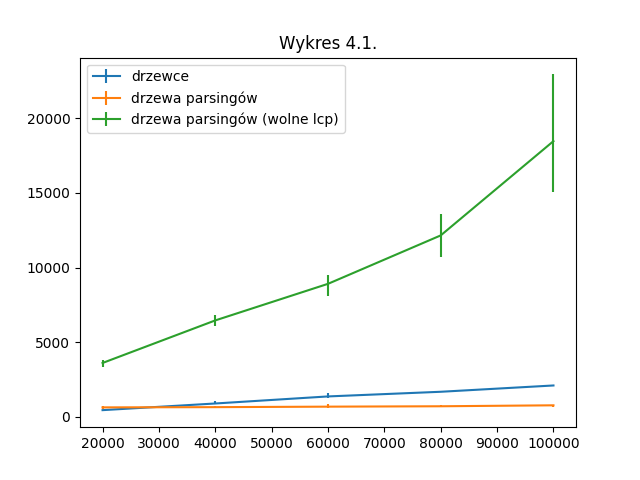
\includegraphics[width=\textwidth]{tablica1.png}
\end{center}

Na podstawie wykresu 4.1 widzimy, że najszybciej działa program implementujący drzewa parsingów. Jest to pocieszające, bo algorytm ten ma asymptotycznie o logarytm lepszą złożoność na każdym zapytaniu. Jednakże tak jak mogliśmy się spodziewać, za implementacją tego algorytmu kryje się znacznie większa stała niż w przypadku drzew zbalansowanych. Mimo to już dla miliona zapytań różnica czasowa między czasem działania struktury drzew parsingów, a drzew zbalansowanych różni się o ponad sekundę. Aby lepiej zobrazować różnicę między dwoma szybkimi rozwiązaniami, przedstawiono wykres 4.2, ponieważ na wykresie 4.1 skalę zaburza czas działania drzew parsingów z wolnym \texttt{lcp}, który jest bardzo duży. Widać na tym przykładzie dobrze skalę różnicy ukrytej stałej w implementacji drzew zbalansowanych i drzew parsingów, bo oba rozwiązania mają taką samą asymptotyczną złożoność czasową.

\begin{center}
    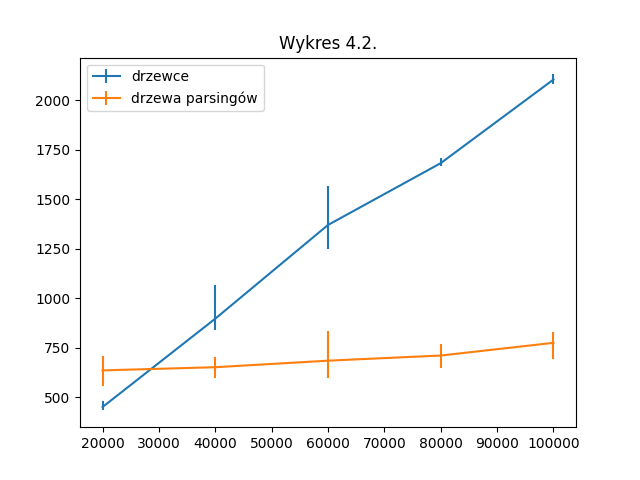
\includegraphics[width=\textwidth]{tablica2.png}
\end{center}

Wykonywanie naprzemiennie losowych poprawnych operacji na słowniku oraz zapytań jest przedstawione na kolejnych dwóch wykresach. Tym razem wyniki eksperymentów są inne. Najszybciej działa program implementujący drzewa zbalansowane. W przypadku gdy większość zapytań nie stanowi zapytanie \texttt{lcp} lub \texttt{smaller}, program z drzewami zbalansowanymi zdaje się działać istotnie szybciej. Mały wkład w wynik eksperymentu metod \texttt{lcp} i \texttt{smaller} potwierdza niewielka różnica między dwoma implementacjami drzewa parsingów, mimo że wiemy że różnica czasu działania podanych wyżej funkcji jest naprawdę istotna, bo zauważyliśmy to interpretując eksperyment z tablicą sufiksową. Porównanie obu rozwiązań implementujących drzewa parsingów widzimy na wykresie 4.4.

\begin{center}
    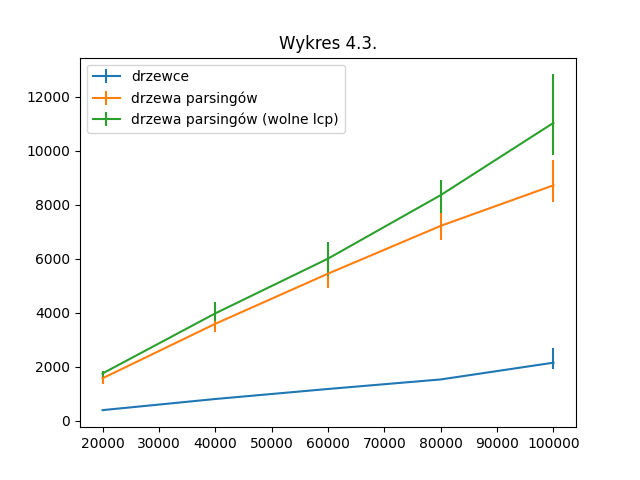
\includegraphics[width=\textwidth]{losowy1.png}
\end{center}

\section{Podsumowanie}

Przeprowadzone eksperymenty potwierdziły, że nawet mimo sporej stałej, algorytm realizujący drzewa parsingów będzie najlepszym wyborem w przypadku gdy korzystając z naszego interfejsu, największą część będą stanowiły zapytania, które są asymptotycznie wolniejsze w pozostałych strukturach. Przy analizie wyników eksperymentu należy uwzględnić dwie rzeczy: podana implementacja drzew parsingów nie jest optymalna, nawet pomijając fakt przejścia ze złożoności typu w.h.p. na złożoność oczekiwaną. Z drugiej strony sama techniczna część implementacji na pewno mogłaby mieć wiele usprawnień, ale miejsce na takie zwykle przychodzi po wielokrotnych implementacjach tej samej struktury. W moim przypadku drzewa zbalansowane implementowałem wiele razy, dlatego znałem techniki pozwalające znacznie poprawić stałą kryjącą się za algorytmem, czego nie mogę powiedzieć o implementacji drzew parsingów, która była przeze mnie tworzona po raz pierwszy. Różnica w stałej, na przykład między operacjami \texttt{split} z interfejsu jest bardzo mocno widoczna na wykresie 4.1, ponieważ wolniejsza wersja drzew parsingów i drzewce implementują dokładnie takie samo wyszukiwanie binarne, zatem cała różnica wynika z funkcji \texttt{split}, a różnica jest bardzo duża. Oczywiście dużym plusem w przypadku drzew parsingów jest brak Monte Carlo, które jest obecne w drzewcach oraz możliwość implementacji w rozsądnym czasie, sporo algorytmów opisywanych w pracach naukowych jest zbyt skomplikowanych do implementacji i używania w praktycznych zastosowaniach, czego nie można powiedzieć o tej strukturze. Myślę, że odpowiednio dopracowana implementacja drzew parsingów może znaleźć swoje miejsce w wielu praktycznych zastosowaniach.

\begin{center}
    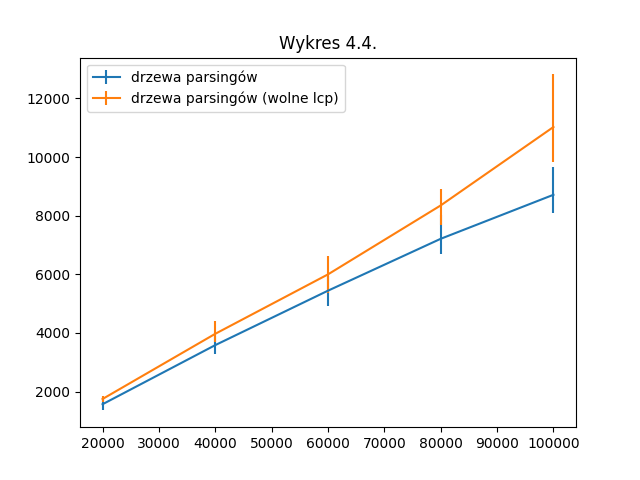
\includegraphics[width=\textwidth]{losowy2.png}
\end{center}

\begin{thebibliography}{1}
\bibitem{paper1}
P. Gawrychowski, A. Karczmarz, T. Kociumaka, J. Łącki i P. Sankowski.
\textit{Optimal Dynamic Strings}.
2016.
\bibitem{paper2}
K. Mehlhorn, R. Sundar i C. Uhrig.
\textit{Maintaining dynamic sequences under equality tests in polylogarithmic time}. 1996.
\end{thebibliography}

\end{document}
